\documentclass[a4paper,11pt,portuguese]{article}
\usepackage{graphicx}
\usepackage{geometry}
\usepackage{hyperref}
\usepackage{float}
\usepackage{enumitem}
\usepackage{listings}
\usepackage{subfig}
\usepackage[portuguese]{babel}

\geometry{margin=1in}


\begin{document}

%%% Identificação %%%

\author{
    Diogo Luís Henriques Costa - 50\% \\
    up201906731
    \and
    Francisco José Barbosa Marques Colino - 50\% \\
    up201905405
}
\title{FEUP -- Programação Funcional e em Lógica \large 2021/2022 \\ \large TP2 -- BreakthroughTanks\_1}
\date{\today}
\maketitle


%%% Instalação e execução %%%
\section{Instalação e execução}

Para a execução deste jogo é necessário o \textit{software} \textit{SICStus Prolog 4.7}. Neste, é necessário incluir o ficheiro
\textit{main.pl} que se encontra na pasta \textit{src} e executar \textit{play.}, a partir  deste ponto o menu 
do jogo fornecerá as instruções de uso necessárias.


%%% Descrição do jogo %%%
\section{Descrição do jogo}

\href{https://boardgamegeek.com/boardgame/321224/breakthrough-tanks}{BreakthroughTanks}
é um jogo de tabuleiro de estratégia por turnos. É jogado por 2 jogadores oponentes, cada 
um controlando um conjunto de peças sobre um tabuleiro quadrangular, de dimensões pares, que podem variar
de 6x6 até 26x26. O objetivo do jogo é ser o primeiro a ter uma peça na linha mais distante, ou seja, a casa do oponente. 

\subsection{Peças}

\noindent Existem 3 tipos de peças:

\begin{enumerate}[topsep=4pt,itemsep=2pt]
    \item \textit{Medium tank}
    \item \textit{Heavy tank}
    \item \textit{Tank destroyer}
\end{enumerate}

\begin{figure}[H]
    \centering
    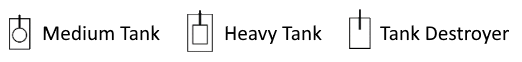
\includegraphics[width=0.5\textwidth]{imgs/pecas.png}
    \caption{Tipo de peças.}
    \label{fig:pecas}
\end{figure}

\noindent Num tabuleiro 8x8, cada jogador começa com 2 \textit{heavy tanks}, 4 \textit{tank destroyers}
e 10 \textit{medium tanks}. A sua disposição inicial no tabuleiro é a seguinte:

\begin{figure}[H]
    \centering
    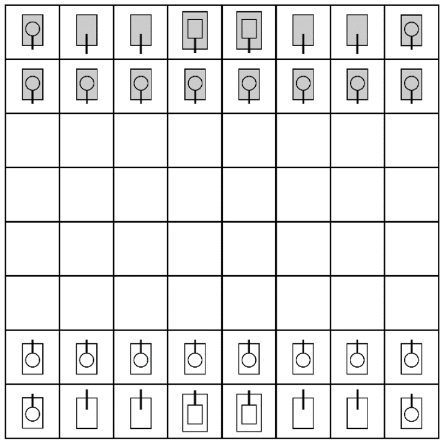
\includegraphics[width=0.25\textwidth]{imgs/board.png}
    \caption{Disposição inicial do tabuleiro.}
    \label{fig:board}
\end{figure}

\noindent Em todas as dimensões de tabuleiro, cada jogador fica com as linhas mais próximas de si completas com \textit{tanks}.
A 2ª linha mais próxima fica completa com \textit{medium tanks} e a linha mais próxima varia no número
de \textit{tank destroyers}, sendo que eles se posicionam em ambos os lados dos \textit{heavy tanks}.
Em todas as dimensões o posicionamento e quantidade (2) de \textit{heavy tanks} mantém-se.

\subsection{Movimentação simples}
Em cada turno uma peça faz uma movimentação simples ou executa uma captura. No caso 
da movimentação, esta é igual para todas as peças: uma unidade para a frente, ou uma 
unidade para uma das diagonais da frente.

\begin{figure}[H]
    \centering
    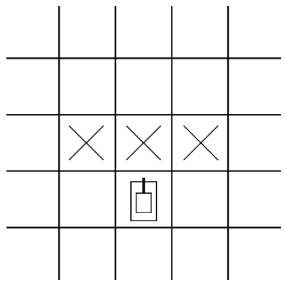
\includegraphics[width=0.2\textwidth]{imgs/movement.png}
    \caption{Movimentação.}
    \label{fig:movemente}
\end{figure}

\subsection{Captura}
Quando uma peça \textbf{A} captura uma peça inimiga \textbf{B}, a peça \textbf{B} é retirada do tabuleiro
e a peça \textbf{A} passa a ocupar o lugar anteriormente ocupado por \textbf{B}. 

\begin{enumerate}[topsep=4pt,itemsep=2pt]
    \item O \textit{Medium tank} captura da mesma forma que se move.
    \item O \textit{Heavy tank} captura 2 casas tanto para a frente 
    como nas diagonais da frente.
    \item O \textit{Tank destroyer} captura 2 casas para a frente.
\end{enumerate}

\noindent Neste jogo, o jogador não é obrigado a capturar caso seja possível.
Ele pode escolher capturar, ou mover a peça em causa de forma normal, ou até
mesmo mover outra peça.

\begin{figure}[H]
    \centering
    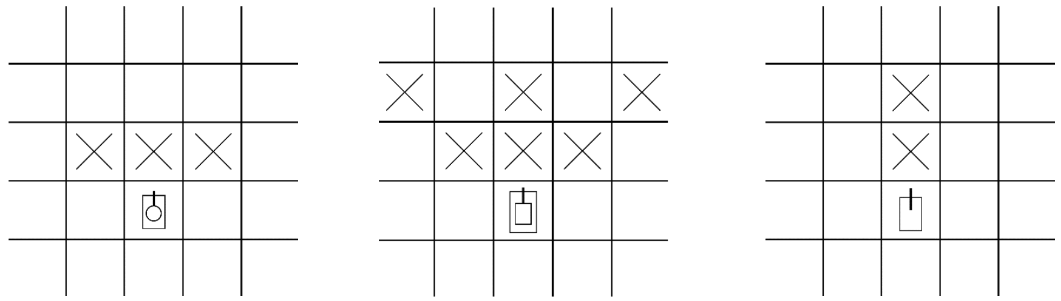
\includegraphics[width=0.5\textwidth]{imgs/capture.png}
    \caption{Captura de peças.}
    \label{fig:capture}
\end{figure}

\subsection{Fim do jogo}

O jogo acaba quando um jogador consegue chegar com uma peça sua à linha mais
afastada, ou seja, à linha mais próxima do oponente.
De notar que, caso um jogador fique sem peças, o seu adversário vence também o jogo.


%%% Lógica do jogo %%%
\section{Lógica do jogo}

    %%% Representação interna do estado do jogo %%%
    \subsection{Representação interna do estado do jogo}

    O estado do jogo, \textit{GameState}, é representado por: Turn-Board. Por sua vez, Turn pode ser ``top" ou ``bot"
    e Board é uma lista de listas de inteiros representando o tabuleiro.  

    \noindent O board é preenchido da seguinte forma:
    \begin{itemize}[topsep=4pt,itemsep=2pt]
        \item  0 -- Espaço vazio
        \item  1 -- \textit{Medium Tank} do \textit{bot player}
        \item  2 -- \textit{Heavy Tank} do \textit{bot player}
        \item  3 -- \textit{Tank destroyer} do \textit{bot player}
        \item -1 -- \textit{Medium Tank} do \textit{top player}
        \item -2 -- \textit{Heavy Tank} do \textit{top player}
        \item -3 -- \textit{Tank destroyer} do \textit{top player}
    \end{itemize}  

    \vspace{1em}
    Desta forma, cada tipo de \textit{tank}: \textit{medium tank, heavy tank, tank destroyer}, pode ser obtido
    recorrendo ao valor absoluto. Por outro lado, as peças de cada jogador distinguem-se pelo sinal: as peças do \textit{top player}
    têm representação interna negativa enquanto que as peças do \textit{bot player} têm representação positiva.

    \vspace{2em}
    \noindent Exemplos de estados de jogo:
    
    \subsubsection{Estado de jogo inicial, 8x8}
\begin{lstlisting}[language=prolog]
bot-[
        [ -1, -3, -3, -2, -2, -3, -3, -1],
        [ -1, -1, -1, -1, -1, -1, -1, -1],
        [  0,  0,  0,  0,  0,  0,  0,  0],
        [  0,  0,  0,  0,  0,  0,  0,  0],
        [  0,  0,  0,  0,  0,  0,  0,  0],
        [  0,  0,  0,  0,  0,  0,  0,  0],
        [  1,  1,  1,  1,  1,  1,  1,  1],
        [  1,  3,  3,  2,  2,  3,  3,  1]
    ]
\end{lstlisting}

    \noindent De modo a obter este estado, recorre-se ao predicado
    \textit{initial\_state(+Size, -GameState)} definido no ficheiro \textit{representation.pl}:
\begin{lstlisting}[language=prolog]
% initial_state(+Size, -GameState)
initial_state(Size, bot-Board):-
    between(6, 26, Size),
    even(Size),
    get_initial_board(Size, Board).
\end{lstlisting}


    \subsubsection{Estado de jogo intermédio, 8x8}
\begin{lstlisting}[language=prolog]
top-[
        [  0,  0,  0,  0,  0, -3, -3, -1],
        [  0,  0,  0,  0, -1, -1, -1, -1],
        [ -1,  2,  0,  0,  0,  0,  0,  0],
        [  0,  0,  0,  0, -2,  0,  0,  0],
        [  0,  0,  0,  0,  0,  0,  0,  0],
        [  0,  0,  0,  1,  0,  0,  0,  0],
        [  0,  0,  0,  0,  1,  1,  1,  1],
        [  1,  0,  0,  0,  0,  3,  3,  1]
]
\end{lstlisting}

    \subsubsection{Estado de jogo final, 8x8}
\begin{lstlisting}[language=prolog]
top-[
        [  2,  0,  0,  0,  0, -3, -3, -1],
        [  0,  0,  0,  0,  0, -1, -1, -1],
        [ -1,  0,  0, -1,  0,  0,  0,  0],
        [  0,  0,  0,  0,  0,  0,  0,  0],
        [  0,  0,  0,  1,  0,  0,  0,  0],
        [  0,  0,  0,  0,  0,  0,  0,  0],
        [  0,  0,  0,  0,  1,  1,  1,  1],
        [  1,  0,  0,  0,  0,  3,  3,  1]
    ]
\end{lstlisting}

    \noindent Neste caso o vencedor foi o \textit{bot player} dado que conseguiu
    alcançar a linha mais próxima do oponente com um dos seus \textit{tanks}.

    %%% Visualização do estado do jogo %%%
    % TODO acrescentar cenas de menu (?)
    % TODO acrescentar que dá para escolher que tipo de jogador é tanto o top como bot...
    \subsection{Visualização do estado do jogo}

    Os predicados de visualização do estado de jogo estão definidos no ficheiro
    \textit{display.pl}.

    \noindent As peças são representadas da seguinte forma:
    \begin{itemize}[topsep=4pt,itemsep=2pt]
        \item ` ' -- Espaço vazio
        \item `M' -- \textit{Medium Tank} do \textit{bot player}
        \item `T' -- \textit{Heavy Tank} do \textit{bot player}
        \item `D' -- \textit{Tank destroyer} do \textit{bot player}
        \item `m' -- \textit{Medium Tank} do \textit{top player}
        \item `t' -- \textit{Heavy Tank} do \textit{top player}
        \item `d' -- \textit{Tank destroyer} do \textit{top player}
    \end{itemize}  

    \noindent O predicado \textit{display\_game(+GameState) } é usado para visualizar
    o estado do jogo, descrito na secção anterior:

\begin{lstlisting}[language=prolog]
% display_game(+GameState)
display_game(Turn-Board):-
    print_board(Board),
    write('Current player: '),
    write(Turn),
    nl.
\end{lstlisting}

    \noindent Este predicado é flexível uma vez que permite visualizar tabuleiros
    de diversos tamanhos:

    \begin{figure}[H]
        \centering
        \subfloat[\centering Tabuleiro 8x8.]{{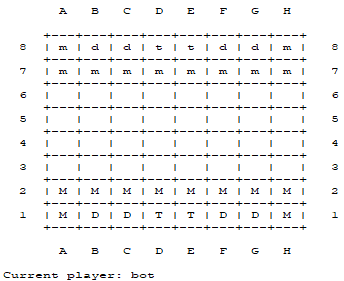
\includegraphics[width=0.4\textwidth]{imgs/board_8_initial.png} }}
        \qquad
        \subfloat[\centering Tabuleiro 12x12.]{{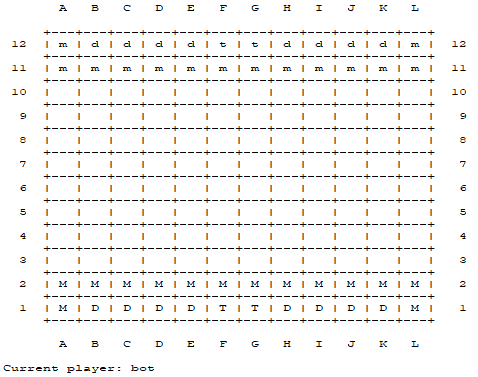
\includegraphics[width=0.4\textwidth]{imgs/board_12_initial.png} }}
        \caption{Visualização do estado jogo.}
        \label{fig:board_view}
    \end{figure}
    
    \noindent O predicado \textit{print\_board(+Board) } é usado para visualizar
    o tabuleiro do jogo sendo a sua definição modular já que ele recorre a predicados
    tais como:

    \begin{itemize}[topsep=4pt,itemsep=2pt]
        \item \textit{print\_board\_line(+Line, +Number) }
        \item \textit{print\_board\_horizontal\_separator(+Size) }
        \item \textit{print\_nav\_horizontal(+Size) }
    \end{itemize}

    \noindent Esta separação de responsabilidades parametrizável com \textit{Size}, permite
    a flexibilidade quanto ao tamanho.

    \noindent Quanto ao \textit{input}, os predicados estão definidos no ficheiro \textit{input.pl},
    sendo estes os principais:

    \begin{itemize}[topsep=4pt,itemsep=2pt]
        \item \textit{read\_move(+Size, -Move) }
        \item \textit{read\_coords(+Size, -ColumnIndex, -RowIndex) }
        \item \textit{read\_valid\_column\_index(+Size, -ColumnIndex) }
        \item \textit{read\_valid\_row\_index(+Size, -RowIndex) }
        \item \textit{read\_letter(-LetterCode) }
        \item \textit{read\_number(-Number) }
    \end{itemize}
    
    \noindent De notar que a este nível, a validação de \textit{input} é feita quanto
    ao tipo de caracteres prentendido (letras ou dígitos) e tamanho do \textit{Board},
    ou seja, que não se seleciona uma posição fora do tabuleiro. A verificação de
    validade da jogada é feita ao nível do módulo lógico que valida as jogadas e caso
    não seja válida, o \textit{backtracking} inerente à execução de \textit{Prolog}
    faz com que o \textit{user} volte a ter que inserir uma jogada.

    De notar que \textit{read\_number(-Number)} lê e valida um número, com número
    indefinido de dígitos, seguido de um \textit{enter} enquanto que
    \textit{read\_letter(-LetterCode)} lê e valida uma letra, seja ela maiúscula
    ou minúscula, seguida de um \textit{enter}. Isto permite que o utilizador,
    quando pretende selecionar uma coluna tanto possa escrever com maiúsculas
    como mínusculas.

    %%% Execução de jogadas %%%
    \subsection{Execução de jogadas}

    O predicado \textit{move(+GameState, +Move, -NewGameState)} , definido no ficheiro
    \textit{logic.pl} é o responsável pela validação e execução de uma jogada:

\begin{lstlisting}[language=prolog]
% move(+GameState, +Move, -NewGameState)
move(Turn-Board, Move, NewTurn-NewBoard):-
    valid_move(Turn-Board, Move),
    do_valid_move(Board, Move, NewBoard),
    switch_turn(Turn, NewTurn).
\end{lstlisting}

    \noindent A validação de uma jogada, efetuada por
    \textit{valid\_move(+GameState, ?Move) } faz-se da seguinte forma:

    \begin{enumerate}[topsep=4pt,itemsep=2pt]
        \item Obtém-se o elemento na posição inicial
        \item Verfica-se se é um \textit{tank} do jogador que está a jogar
        \item Obtém-se o elemento na posição final
        \item Faz-se a subtração das coordenadas para obter a translação associada
        \item Verifica-se se a posição final não tem um \textit{tank} do jogador que
        está a jogar
        \item Verifica-se se a translação do movimento é válida dado o \textit{tank}
        da posição inicial e o elemnto (\textit{tank} inimigo ou espaço vazio) da posição final
    \end{enumerate}

    \noindent De notar que, com o objetivo de reutilizar código, normalizaram-se as jogadas
    para o \textit{bot player}. Exemplo disso é o facto de, caso seja o \textit{top player}
    a jogar, a translação associada ao movimento é refletida horizontalente de modo a utilizar
    os mesmos predicados para ambos os jogadores. Também os \textit{tanks} são tomados pelo seu
    valor absoluto (o \textit{bot player} tem os seus \textit{tanks} representados por números
    positivos).

    Após saber que a jogada é válida, para executar uma jogada basta colocar um \textit{0}
    na posição inicial e colocar na posição final o número (\textit{tank}) que estava na
    posição inicial recorrendo-se ao predicado
    \textit{matrix\_put\_at(+Matrix, +[C,L], +Elem, -ModifiedMatrix) } definido no ficheiro
    \textit{utils.pl}.


    %%% Final de jogo %%%
    \subsection{Final de jogo}

    O predicado \textit{game\_over(+GameState, -Winner)} é usado para a deteção do final
    do jogo e atribuição do vencedor. Um jogador ganha se o seu oponente não tiver mais 
    peças para jogar, \textit{not(matrix\_has\_range(Board, positive))} e 
    \textit{not(matrix\_has\_range(Board, negative))}, ou, no caso do \textit{top}, se
    tiver uma peça sua na última linha do \textit{board}, a linha mais próxima do inimigo, 
    \textit{min\_member(Min, BotRow)}, e no caso do \textit{bot} se tiver uma peça sua
    na primeira linha do \textit{board}, a linha mais próxima do inimigo, 
    \textit{max\_member(Max, TopRow)}.


    %%% Lista de jogadas válidas %%%
    \subsection{Lista de jogadas válidas}

    O predicado \textit{valid\_moves(+GameState, -ListOfMoves)} é usado para obter a
    lista de jogadas válidas e está definido no ficheiro \textit{logic.pl}:

\begin{lstlisting}[language=prolog]
% valid_moves(+GameState, -ListOfMoves)
valid_moves(GameState, ListOfMoves):-
    findall(Move, valid_move(GameState, Move), ListOfMoves).
\end{lstlisting}

    \noindent Este predicado tem uma definição curta dado que faz uso do predicado
    \textit{valid\_move(+GameState, ?Move) } (com definição descrita na secção de
    \textit{Execução de jogadas}) e recorre a \textit{findall(Term, Goal, List)}
    para obter uma listagem de todas as jogadas válidas.


    %%% Avaliação do Estado do Jogo %%%
    \subsection{Avaliação do Estado do Jogo}

    A avaliação do estado de jogo, \textit{value(+GameState, +Player, -Value)}, é feita
    para cada jogador tendo em conta o tabuleiro todo usando os seguintes fatores:
    \begin{itemize}
        \item Tipo de \textit{tank}
        \begin{itemize}
            \item o \textit{medium tank} vale 100 pontos
            \item o \textit{tank destroyer} vale 125 pontos
            \item o \textit{heavy tank} vale 150 pontos
        \end{itemize}
        \item Distância à sua base
    \end{itemize}

    O valor atribuído a cada \textit{tank} é calculado com a multiplicação do valor do seu tipo
    pelo fator da distância que é $ 2^{dist\_to\_home} $, sendo que a \textit{dist\_to\_home}
    é o número de casas a que o \textit{tank} se encontra do jogador ao qual pertence.
    O valor final do tabuleiro é calculado através da soma do valor de todos os \textit{tanks}
    do jogador para o qual está a ser calculada a jogada (\textit{top} ou \textit{bot}) e é
    depois subtraído o valor de todos os \textit{tanks} que pertencem ao seu oponente.


    %%% Jogada do Computador %%%
    \subsection{Jogada do Computador}

    O jogo oferece dois níveis de dificuldade do computador como inimigo.
    No nível 1 o computador faz uma jogada aleatória que seja válida, no nível 2
    o computador escolhe a jogada que lhe dá mais vantagem, fazendo as previsões
    numa distância de uma jogada (algoritmo míope). Para este efeito são simuladas todas
    as jogadas possíveis que o computador pode fazer e é calculado o valor de cada, através 
    do método de avaliação mencionado na secção anterior, e é então escolhida a jogada que obtém 
    um estado de jogo com maior valor, \textit{choose\_move(+GameState, +Level, -Move)}, no
    caso de empate é escolhido um dos melhores resultados aleatoriamente. 



%%% Conclusões %%%
\section{Conclusões}

Foi implementado em \textit{Prolog} um jogo de tabuleiro a 2 jogadores com tamanho de tabuleiro
variável. Os jogadores tanto podem ser humanos como \textit{PC} sendo que neste último caso
existem dois níveis associados. Assim, todos os objetivos deste trabalho foram alcançados. \par

Caso se pretendesse desenvolver e adicionar complexidade ao jogo, duas possíveis alterações
seriam a possíbilidade de configurar a disposição inicial do tabuleiro e adicionar mais níveis
ao jogador \textit{PC} fazendo uso, por exemplo, do algorítmo \textit{minimax}. \par

A realização deste trabalho permitiu fazer um estudo mais imersivo de \textit{Prolog} que não
seria possível realizando apenas os exercícios das aulas práticas.


%%% Bibliografia %%%
\section{Bibliografia}

\subsection{Página do jogo}
\href{https://boardgamegeek.com/boardgame/321224/breakthrough-tanks}{https://boardgamegeek.com/boardgame/321224/breakthrough-tanks}


\end{document}
